%-----------------------------------------------------------------------
% Beginning of chap1.tex
%-----------------------------------------------------------------------
%
%  Use this file as a model for a chapter; DO NOT START BY removing its
%  contents and filling in your own text.
% 
%%%%%%%%%%%%%%%%%%%%%%%%%%%%%%%%%%%%%%%%%%%%%%%%%%%%%%%%%%%%%%%%%%%%%%%%

\chapter[INTRODUCTION]{Introduction}

%If a chapter command is immediately followed by a section command 
% add the following line to preserve the space
\vspace{-12pt}
\section{Background}

Although inland fresh waters cover ~1\% of the Earth's surface, they disproportionately provide valuable services such as water purification, irrigation, flood control, support biodiversity, nutrient cycling, and carbon storage \cite{williamson_lakes_2008, palmerEcologyHeartbeatEcosystems2012}. Many of these ecosystem services are linked to stream flow regime. Global climate models predict many regions will become more arid. Annual precipitation will decrease, while timing and intensity of precipitation events will increase \cite{IPCC}. With increases in human populations, more land is expected to be urbanized or converted for agricultural use. This can lead to more impervious surfaces, increased nutrient loads, and increased turbidity. Ecosystem functions such as nutrient cycling, and carbon storage respond to changes in a stream’s watershed, such as native vegetation being developed for urban, or agriculture uses; or changes in precipitation regime. Changes in climate and land use affects ecosystem functions of streams \cite{grimm_changing_2008}.


\section{Ecosystem Metabolism}
Ecosystem metabolism is a measure of ecosystem function and modulates nutrient and organic matter cycling \cite{izagirre_environmental_2008, williamson_lakes_2008}. Ecosystem metabolism encompasses gross primary production (GPP), the fixation of inorganic carbon to organic carbon via photosynthesis, and ecosystem respiration (ER), the mineralization of carbon by autotrophs and heterotrophs. A majority of our knowledge on ecosystem metabolism in rivers comes from small rivers with discharge less than 0.1 m$^3$ s$^{-1}$, with active benthic zones, rather than large rivers with planktonic zones \cite{hall_metabolism_2016, bernhardt_metabolic_2018}. 
Both proximal and distal drivers control GPP and ER. Proximal drivers include light, temperature, nutrients, hydrology, and organic matter, whereas distal drivers include land use, climate, soil, vegetation, and disturbance \cite{izagirre_environmental_2008, bernot_inter-regional_2010}. 

GPP and ER can be estimated from diel changes in dissolved oxygen concentrations \cite{odum_primary_1956}. GPP is a positive flux because oxygen is released via photosynthesis, and ER, a negative flux because oxygen is consumed during respiration. Net ecosystem production (NEP) is the sum of GPP and ER fluxes. Ecosystems with a positive NEP are autotrophic, because GPP exceeds ER, whereas ecosystems with negative NEP are heterotrophic, because GPP is less than ER \cite{lovett_is_2006}. 

With advances in technology, methods of measuring ecosystem metabolism in streams have changed since the first introduction of open-channel ecosystem metabolism by Odum (1956). Historically, due to measurement constraints, ecosystem metabolism was most often measured on clear weather days for short time periods \cite{odum_primary_1956, bernhardt_metabolic_2018}. Using Odum’s original open-channel metabolism method involved collecting samples every 2-4 hours and estimating the dissolved oxygen with titration \cite{odum_primary_1956}. Following Odum’s method, the first generation of stream sensors to continuously measure dissolved oxygen were developed. Because these sensors were expensive and drifted, they were deployed for short time periods (e.g., 2-3 days) during stable stream flow conditions \cite{bernhardt_metabolic_2018}. However, with advanced sensor technology and computational power, in the last decade we have been able to obtain high-frequency time series of stream water dissolved oxygen and temperature data, ranging from months to years, to calculate ecosystem metabolism. These high frequency estimates of ecosystem metabolism have led to insight into the controls of GPP and ER in streams \cite{beaulieu_continuous_2013, arroita_twenty_2019}.


\section{Ecosystem Metabolism Drivers}

With the insight into controls of GPP and ER, we are beginning to parse out direct and indirect drivers of ecosystem metabolism \cite{bernot_inter-regional_2010, fus_land_2017}. Proximal drivers of ecosystem metabolism, such as light and nutrient concentrations, directly drive changes in rates of ecosystem metabolism, while distal drivers, such as precipitation regimes and watershed land use, indirectly drive changes in ecosystem metabolism by driving changes in proximal drivers (Figure~\ref{fig:concept}).

\subsection{\textit{Proximal Drivers}}
Light controls GPP from daily to seasonal time-scales, as GPP is positively correlated with light availability \cite{mulholland_inter-biome_2001, roberts_multiple_2007, beaulieu_continuous_2013}. For example, streams with little to no riparian vegetation, such as those flowing through urban and agricultural areas, have more light reaching stream primary producers, which drives greater fluxes of GPP when compared to their forested counterparts \cite{bernot_inter-regional_2010, beaulieu_continuous_2013, alberts_watershed_2017}. Across 72 streams in the United States and Puerto Rico, urban and agricultural streams had a 2-fold increase in GPP vs reference (i.e., non-agriculture and non-urban) streams with riparian vegetation, that was attributed to increased nutrients and light \cite{bernot_inter-regional_2010}. In an intermittent suburban stream, light was found to be the primary driver of increased GPP despite increased nutrient concentrations \cite{beaulieu_continuous_2013}. In a semi-arid stream in Nevada, with little riparian vegetation and high light, light was also attributed to high levels of GPP \cite{davis_high_2012}. Even in forested streams, seasonality of leaf cover drives the temporal pattern of GPP. In Walker Branch, a low-order, forested stream located in Tennessee, rates of GPP peaked in spring prior to leaf out but then declined as the canopy closed in summer and fall seasons \cite{roberts_multiple_2007, alberts_watershed_2017}.

Besides canopy cover, factors such as turbidity and slope control light availability to stream ecosystems \cite{hall_turbidity_2015, blaszczak_scoured_2019}. Increasing turbidity within a stream results in less light reaching the primary producers, thus decreasing GPP. Turbidity may have a seasonal component, increasing during rainy seasons and resulting in depressed GPP during those time periods \cite{hall_turbidity_2015}. High riparian slopes, incised stream channels, or canyon walls limit light reaching the primary producers due to shading, resulting in reduced GPP \cite{hall_turbidity_2015, blaszczak_scoured_2019}.

Temperature also drives both GPP and ER in streams. GPP is expected to increase with increasing temperatures at approximately half the rate as ER \cite{perkins_consistent_2012}. For instance, in geothermal streams, negative NEP increased exponentially with increasing temperature due to the imbalance of increasing GPP and ER \cite{demars_temperature_2011}. Increasing biomass with increasing temperatures also explained increases in GPP and ER in 12 streams near Reykjavik, Iceland \cite{padfield_metabolic_2017}. The recovery rate of primary producer biomass following disturbance, such as scouring, may be in part dictated by temperature. For example, increased temperature was linked to quick recovery rates of GPP and ER following scouring events in a Swiss sub-alpine stream \cite{uehlinger_resistance_2000}. 
	
Nutrient concentrations and ecosystem metabolism can modulate each other, with low nutrient concentrations suppressing ecosystem metabolism and high nutrient concentrations leading to daily decreases in nutrient concentrations coinciding with higher production. For instance, based on a 20-year ecosystem metabolism record in a Spanish River, ER was reduced 2.5-fold and GPP 1.8-fold after the implementation of a waste water treatment plant and subsequent reduction of nutrient concentrations \cite{arroita_twenty_2019}. If nutrients are limited, GPP and ER will be suppressed. With an excess of nutrients beyond demand, nutrients will be transported downstream \cite{covino_measuring_2018}. Streams with high nutrient loads may have increased ER, which may lead to large fluctuations in oxygen concentrations and may drive streams to become hypoxic \cite{arroita_twenty_2019}. However, in 72 streams across the United States and Puerto Rico using short-term ecosystem metabolism estimates (e.g. 24-48hr), multiple regression models revealed weak relationships between nutrient concentrations and GPP and ER \cite{bernot_inter-regional_2010}. As you move from a forested stream to one with increasing urban or agricultural land use, you can expect to see an increase in nutrients from anthropogenic runoff \cite{bernot_nutrient_2006, fus_land_2017}. These increased nutrients could increase rates of ecosystem metabolism.

Dissolved organic matter (DOM) can be a strong driver of ER. DOM in aquatic ecosystems can originate from autochthonous sources such as benthic biofilms, phytoplankton, and macrophytes or allochthonous sources, such as soils and leaf litter \cite{bertilsson_supply_2003, fus_land_2017, wong_sources_2010}. DOM can also vary seasonally. In areas with deciduous vegetation, allochthonous sources dominate in fall and winter, with increasing leaf litter entering the streams. In comparison, autochthonous sources dominate in the summer \cite{aitkenhead-peterson_sources_2003}. In 33 Austrian streams, autochthonous DOM was found in urban and agricultural streams, while allochthonous DOM was found in forested streams \cite{fus_land_2017}. DOM from autochthonous and allochthonous sources vary in their composition and bioavailability. DOM from autochthonous sources has a smaller molecular weight and less aromaticity than DOM from allochthonous sources, and is also more bioavailable (i.e. easily consumed by microbes) \cite{wong_sources_2010}. DOM that is more bioavailable is able to fuel microbes resulting in higher fluxes of ER \cite{fus_land_2017}. DOM quantity and quality are also affected by land use of the watershed. For instance, watersheds with agriculture in the watershed will have more DOM from agricultural soils, which tend to be rich in organic matter, and could increase ER \cite{fus_land_2017}. Readily labile DOM is able to be quickly mineralized and provides an energy source for microbes resulting in increased ER fluxes, while intermediate labile DOM is able to provide a downstream subsidy potentially fueling downstream ecosystem metabolism \cite{wiegner_contribution_2005}. 

Hydrology is another controlling factor of ecosystem metabolism in streams, exerting both direct and indirect forces. At lower flows, streams are more efficient at transforming nutrients and DOM, however, at higher flows streams transport nutrients and DOM downstream \cite{fisher_temporal_1982, hall_hydrologic_2009}. If nutrients and DOM have shorter residence times, that is at higher stream flows, they are more likely to be transported downstream \cite{creed_regulation_1996, casas-ruiz_tale_2017}. Frequent high flow events may also alter the geomorphology of streams by incising stream banks, and this will indirectly alter flow and light regimes of the stream \cite{blaszczak_scoured_2019}. Streams with highly incised banks will receive less light than in streams without incised banks. Frequent high flow events can also increase turbidity, which will further limit the light available to primary producers \cite{hall_turbidity_2015, blaszczak_scoured_2019}. Streams with seasonal increases in discharge may have primary producers that are adapted to increases in discharge \cite{lytle_adaptation_2004}. For instance, in 10 sub-alpine streams with seasonal high flows, an increase in GPP coincided with snowmelt, but decreased with other scouring events \cite{ulseth_climate-induced_2018}. Hydrology also controls DOM input, with high flows pulsing in large quantities of terrestrial DOM \cite{fasching_hydrology_2016, raymond_hydrological_2016}. The increased flow rapidly shunts DOM downstream, decreases residence time and therefore is exported downstream; with decreased flow, residence time of DOM is increased, and is more likely to increase ER \cite{battin_biophysical_2008, raymond_hydrological_2016}.


\subsection{\textit{Distal Drivers}}
Light, nutrient concentrations, and DOM are dependent on precipitation regimes. Arid streams tend to have less riparian cover than mesic forested streams, thus more light compared to forested streams, which will lead to an increase in GPP \cite{davis_high_2012, hall_turbidity_2015}. Arid streams will also have less nutrient runoff caused by precipitation events than forested streams. Precipitation transports nutrients through the watershed resulting in high nutrient concentrations within streams with increasing stream discharge \cite{house_hysteresis_1998, ulseth_natural_2005}. With less nutrients transported to arid streams, GPP and ER will be suppressed. Forested streams will have an increase in DOM from precipitation events bringing in more terrestrial DOM from leaf litter or flushing DOM from soils, which is then transported downstream, where it can fuel microbes resulting in higher fluxes of ER \cite{sawyer_hydrologic_2014, raymond_hydrological_2016}. However, it is unknown how these drivers, dictated by precipitation, will respond to changes along a precipitation gradient and influence ecosystem metabolism.


These distal drivers are also dependent on watershed land use. Urban and agricultural streams tend to have less riparian vegetation than forested streams \cite{bernot_inter-regional_2010}. Urban and agricultural streams also tend to have higher nutrient loads than unimpacted streams \cite{bernot_inter-regional_2010, alberts_watershed_2017, fus_land_2017}. In six mid-western streams draining row-crop agriculture fields, high rates of GPP and ER were attributed to excess nutrient runoff from fertilizer and increased light availability caused by grass buffer zones \cite{griffithsAgriculturalLandUse2013}. Within 33 Austrian streams, there was no change in the concentration of DOM between urban/agricultural and forested streams, however, the composition of DOM differed with land use \cite{fus_land_2017}. Changes in land cover from forested to urban and agricultural also affects hydrology. Urban streams have more frequent high flows that can cause scouring of the substrate, which may suppress GPP \cite{booth_urbanization_1997, blaszczak_scoured_2019, uehlinger_resistance_2000, uehlingerEcosystemMetabolismDisturbance1998}. 

Light availability, temperature, nutrient concentrations, and DOM are able to directly drive changes in ecosystem metabolism, while precipitation regimes, watershed land use, and hydrology indirectly drive changes in ecosystem metabolism. However, the combined effects of these proximal and distal drivers on rates of ecosystem metabolism, is less understood (Figure \ref{fig:concept}).


\begin{figure}[htb]
\begin{center}
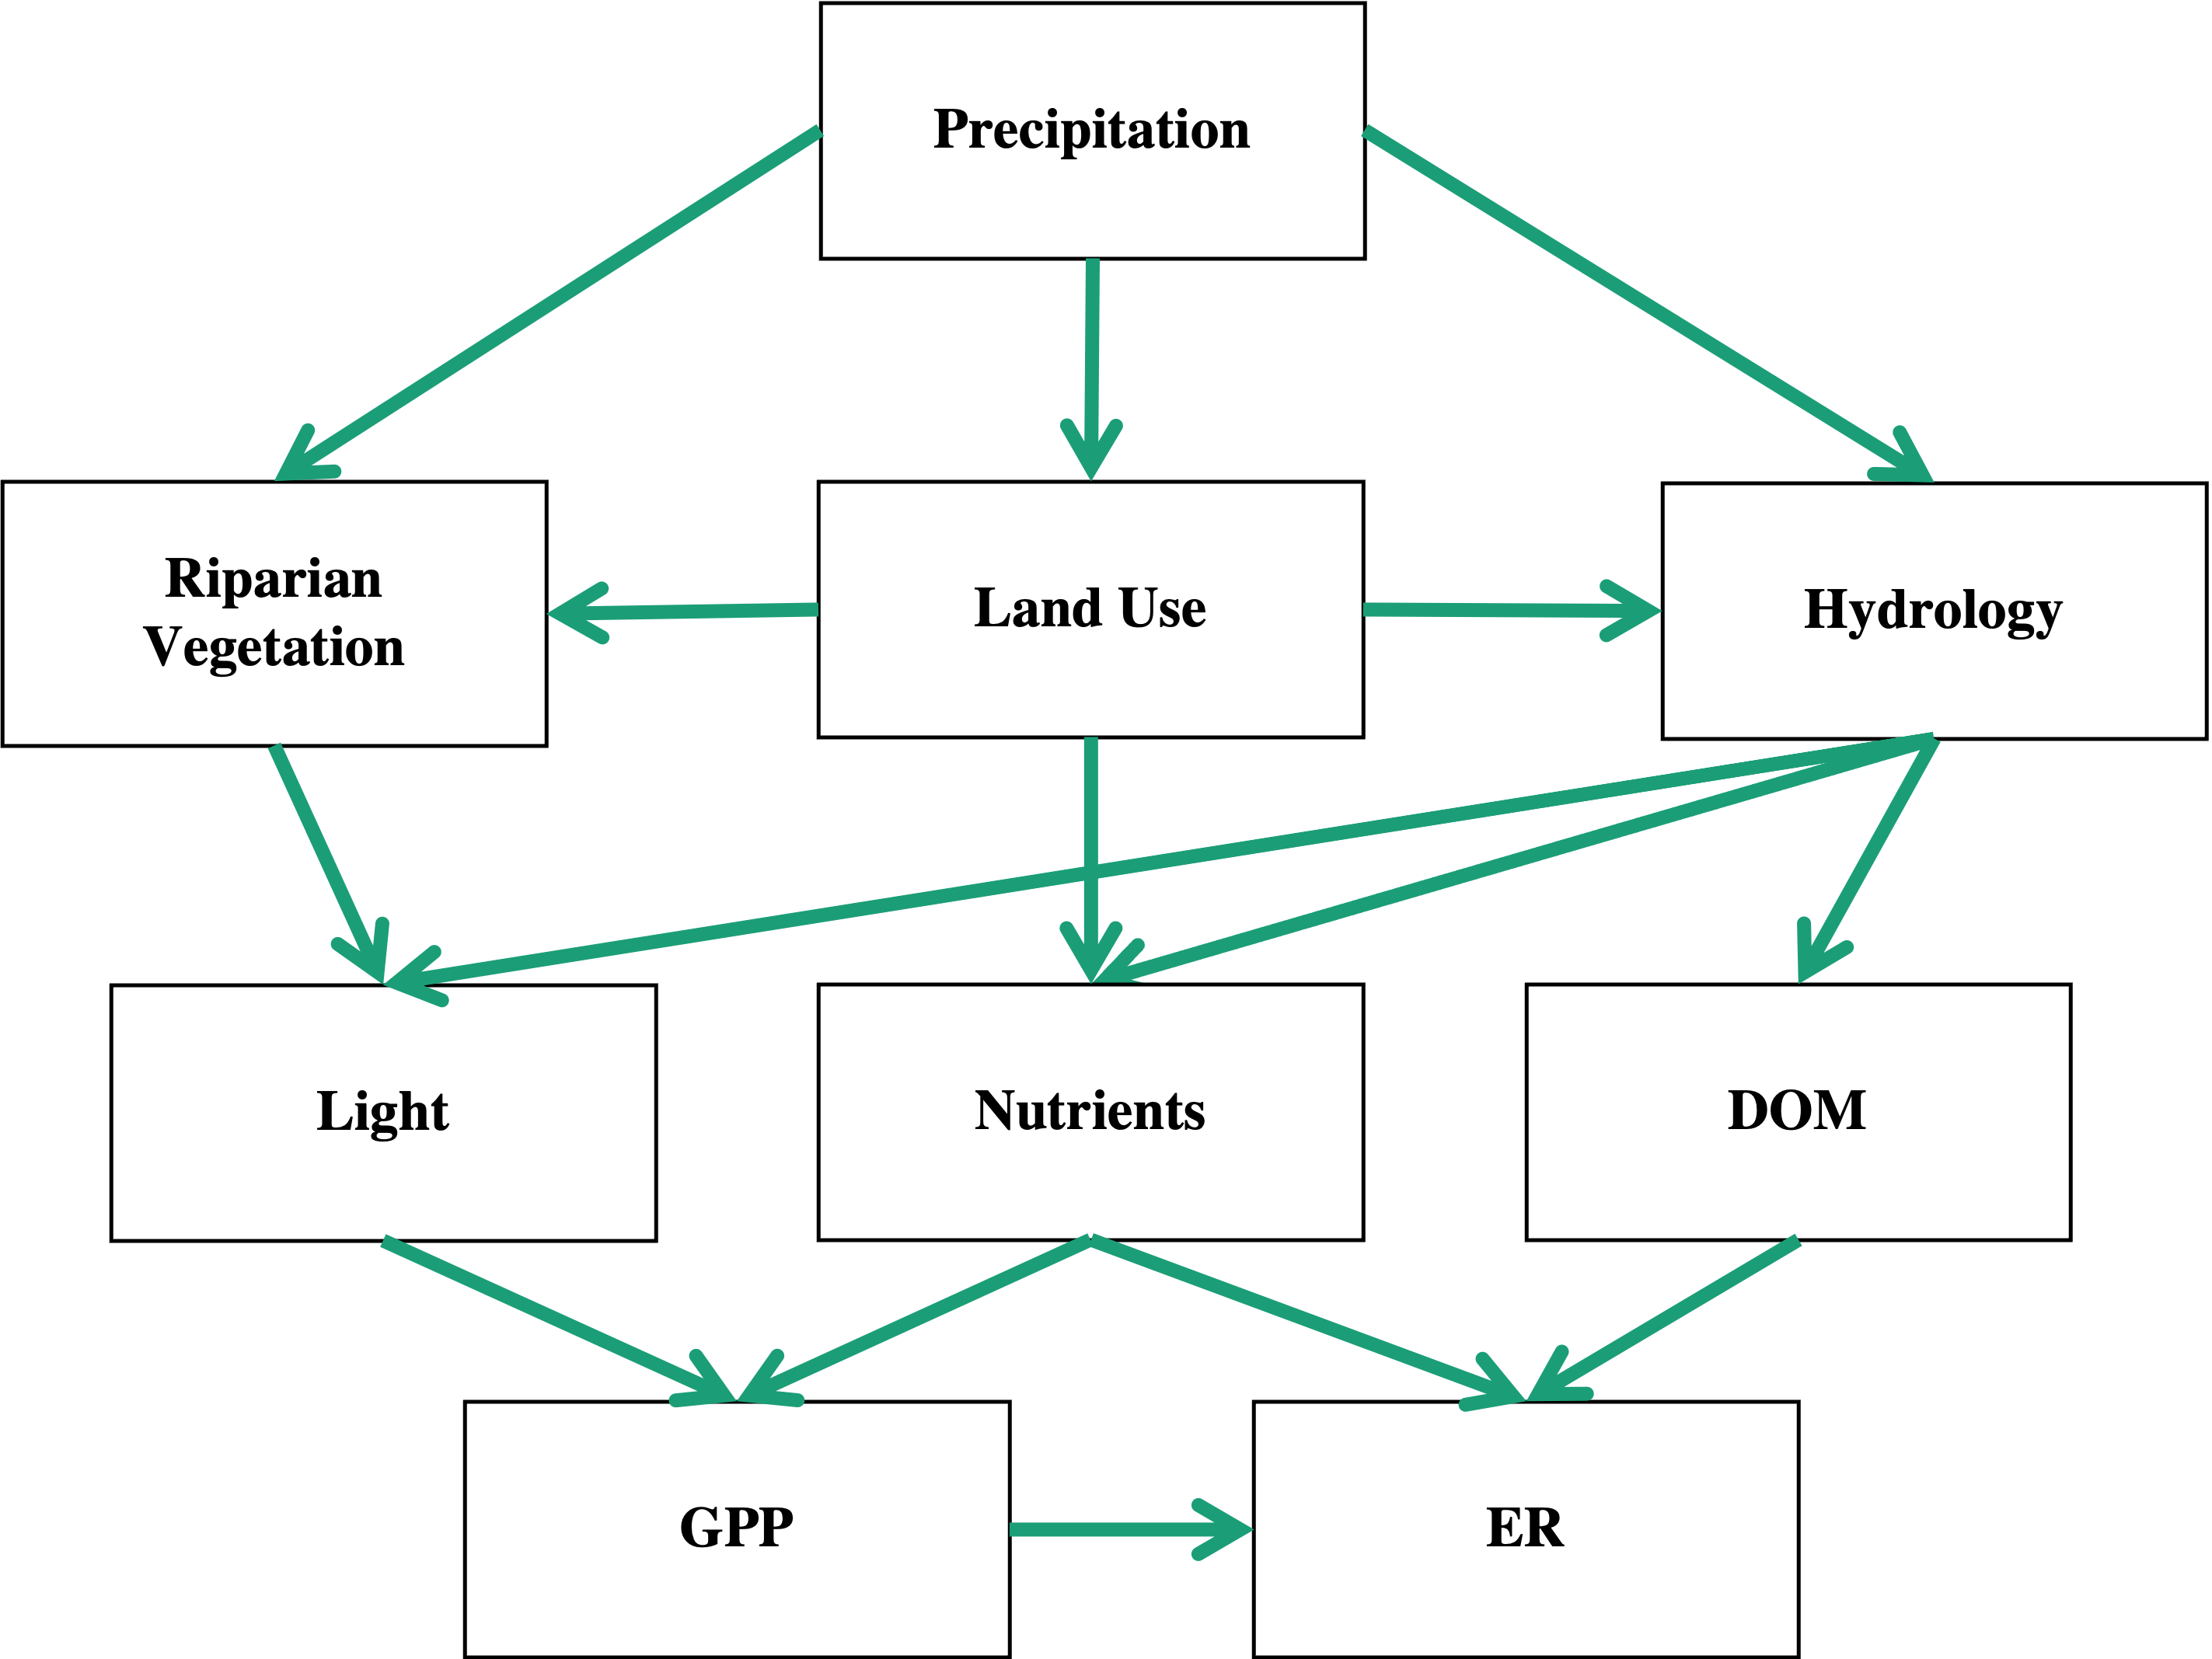
\includegraphics[scale=0.6]{Figs/ConceptDiagGREEN.png}
\caption[Conceptual Diagram]{\textit{Conceptual Diagram}. Conceptual diagram of hypothesized interactions between proximal and distal drivers on ecosystem metabolism.}
\label{fig:concept}
\end{center}
\end{figure}



\section{Research Questions}
\begin{enumerate}
    \item How do changes in light, nutrients, DOC, and hydrology that are driven by precipitation regimes drive patterns of ecosystem metabolism?
    \begin{itemize}
        \item Predictions:
         \begin{itemize}
        \item Increasing precipitation will cause high discharge, which will increase turbidity, attenuate light reaching the benthos, and suppress GPP.
        \item High discharge events will increase scouring or burying events and suppress GPP.
        \item High discharge events will dilute nutrient concentrations and suppress GPP and ER.
        \item As you move from arid to mesic, I expect DOC quantity to increase due to increased precipitation pulsing DOC from the watershed into the streams. Increased DOC will provide more fuel for microbes which will result in increased ER.
    \end{itemize}
    \end{itemize}

    \item How do changes in light, nutrients, DOC, and hydrology that are driven by changes in watershed land use drive patterns of ecosystem metabolism?
    \begin{itemize}
        \item Predictions:
        \begin{itemize}
        \item  Forested land that has been converted into agricultural land will have increased light availability from the removal of non-agricultural vegetation. This will drive an increase in both GPP and ER.
        \item  Forested land that has been converted into agricultural land will have increased nutrients from agricultural runoff, leading to an increase in GPP and ER.
        \item Non-agricultural vegetation will decrease light availability, resulting in suppressed GPP.
    \end{itemize}
    \end{itemize}
    
\end{enumerate}

         
         
         
         



  


\endinput

%-----------------------------------------------------------------------
% End of chap1.tex
%-----------------------------------------------------------------------
